\section{File Extraction and Hash Computation in Zeek}
\subsection{How It Works}
The process of file extraction in Zeek can be summarized as follows:
\begin{enumerate}
  \item \textbf{Event Detection:} Zeek scripts react to network events, such as the presence of a file in the network stream.
  \item \textbf{File Type Identification:} The script identifies the type of the file using its MIME type, enabling appropriate handling.
  \item \textbf{File Handling:} Based on the identified type, the script determines the handling procedure and naming convention for the file.
  \item \textbf{Analyzer Usage:} File analyzers, especially the extraction analyzer, are utilized to automatically save the file to the disk.
  \item \textbf{Extraction Configuration:} Specific parameters, such as the output filename, are defined for the extraction process.

\end{enumerate}

\subsection{File Extraction Script : }

\begin{lstlisting}[language=Python, caption= File EXtraction Script]
event file_sniff(f: fa_file, meta: fa_metadata)
{
    if (!meta?$mime_type) return;
    local filename: string;
    switch (meta$mime_type) {
        case "text/plain":
            print fmt("Detected Text file: %s", f$id);
            filename = fmt("extracted_text_%s.txt", f$id);
            break;
            
        case "text/html":
            print fmt("Detected HTML file: %s", f$id);
            filename = fmt("extracted_html_%s.html", f$id);
            break;
            
        case "image/png":
            print fmt("Detected PNG file: %s", f$id);
            filename = fmt("extracted_png_%s.png", f$id);
            break;

        default:
            return;
    }
    Files::add_analyzer(f, Files::ANALYZER_MD5);
    Files::add_analyzer(f, Files::ANALYZER_EXTRACT, [$extract_filename=filename]);
    
    print fmt("File will be extracted to: %s", filename);
}

event file_hash(f: fa_file, kind: string, hash: string)
{
    if (kind == "MD5")
    {
        print fmt("MD5 hash of file %s: %s", f$id, hash);
    }
}

event zeek_init()
{
    print "Zeek FILE Monitoring Script Initialized.";
}

\end{lstlisting}

\subsection{Script Explanation}
\begin{enumerate}
    \item \textbf{Event Detection} (Line 1) : Triggered by the \texttt{file\_sniff} event, the script processes each file detected in network traffic.
    \item \textbf{MIME Type Check} (Lines 3-19) The script exits the function early if a file does not have a MIME type associated with it.
    \item \textbf{File Classification} (Lines 3-19) : Files are classified based on their MIME type (text, HTML, PNG) and assigned unique filenames.
    \item \textbf{Analyzer Addition} (Lines 24-25) : The script adds MD5 and extraction analyzers for hashing and saving the files, respectively.
    \item \textbf{Extraction Notification} (Line 27) It logs the path where the file will be extracted to.
    \item \textbf{Hash Event} (Lines 30-36) : During the \texttt{file\_hash} event, the MD5 hash of the file is logged.
    \item \textbf{Initialization} (Lines 38-40) : The \texttt{zeek\_init} event signals that the script is ready for file monitoring.
\end{enumerate}

\subsection{Simulation}

We will commence by extracting files through a script that operates on both live network monitoring data and pre-captured pcap files.
\subsubsection{File Extraction from Live Network}
    \begin{itemize}
    \item The initial step involves locating the Zeek executable on the system.
    \end{itemize}
    \begin{figure}[H]
    \centering
    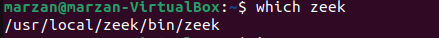
\includegraphics[width=1\linewidth]{images/which_zeek.png}
    \caption{zeek path}
    \label{fig:enter-label}
\end{figure}

     \begin{itemize}
     \item Subsequently, we will identify the active network interface on the machine to monitor the network traffic.
      \end{itemize}
    \begin{figure}[H]
    \centering
    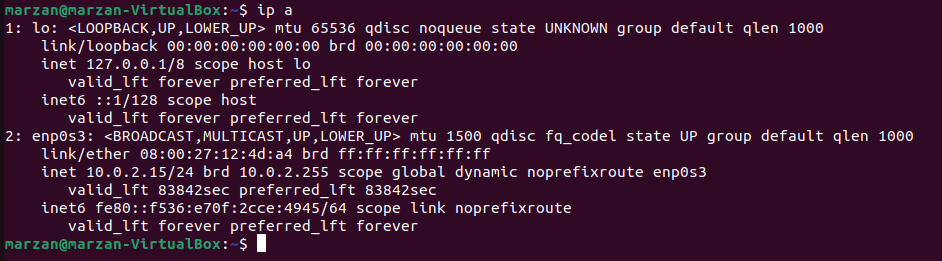
\includegraphics[width=1\linewidth]{images/ipa.png}
    \caption{active network interfaces}
    \label{fig:enter-label}
\end{figure}
\begin{itemize}

\item Following this, we initiate monitoring on the selected interface (enp0s3) using Zeek, which results in the extraction of 2 PDF files from the network traffic
 \end{itemize}
\begin{figure}[H]
    \centering
    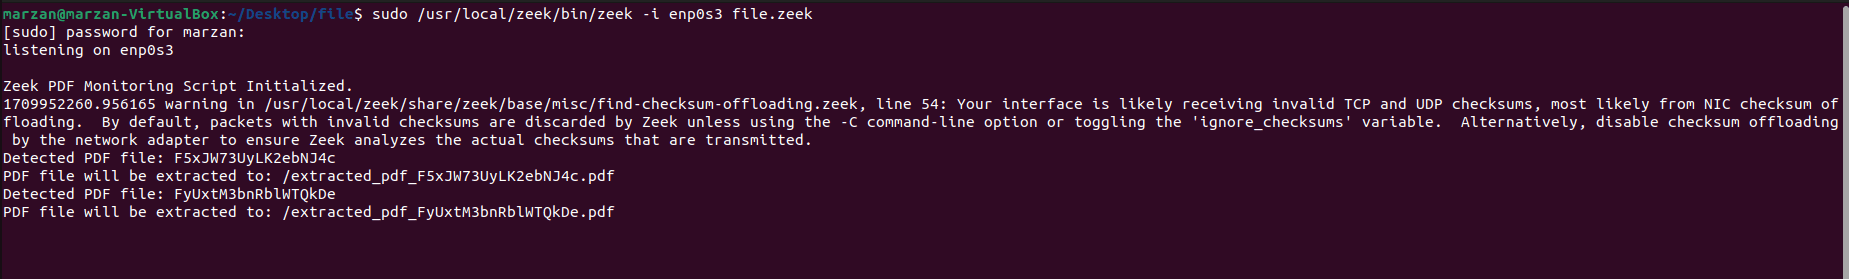
\includegraphics[width=1\linewidth]{images//extract_file/enpos3_file.png}
    \caption{PDF file extraction from live network monitoring}
    \label{fig:enter-label}
\end{figure}

\subsubsection{File Extraction from PCAP file}
\begin{itemize}
\item The same extraction process can be applied to pre-captured pcap files containing file transfer traffic\\\\
For this exercise, a pcap file is available at
PCAP file URL : \url{https://www.cloudshark.org/captures/a9472fbe700a}\\
The file can be downloaded by selecting "Export | Download".\\\\

By analyzing the pcap file with Zeek, we can extract files embedded within the network traffic.
The extracted files, which include a PNG file and a TXT file, are stored in the \textbf{/extract\_files} folder and are named according to their unique identifiers as logged by Zeek.
 \end{itemize}
\begin{figure}[H]
    \centering
    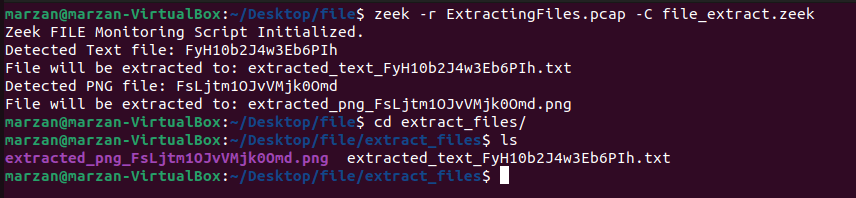
\includegraphics[width=1\linewidth]{images//extract_file/file_extract_1.png}
    \caption{PDF file extraction from pcap file}
    \label{fig:enter-label}
\end{figure}

\begin{itemize}
\item The \textbf{extract\_files} folder contains the two files that were extracted from the pcap file, showcasing Zeek's file extraction capabilities.
 \end{itemize}
\begin{figure}[H]
    \centering
    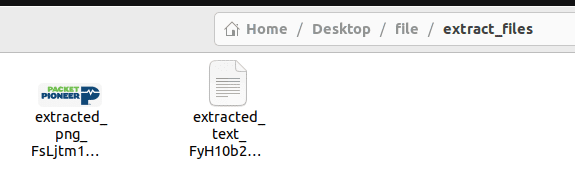
\includegraphics[width=0.5\linewidth]{images//extract_file/file_extract_2.png}
    \caption{Files inside extract\_files folder}
    \label{fig:enter-label}
\end{figure}

\begin{itemize}
\item A PNG file has been successfully extracted from the network traffic.

 \end{itemize}
\begin{figure}[H]
    \centering
    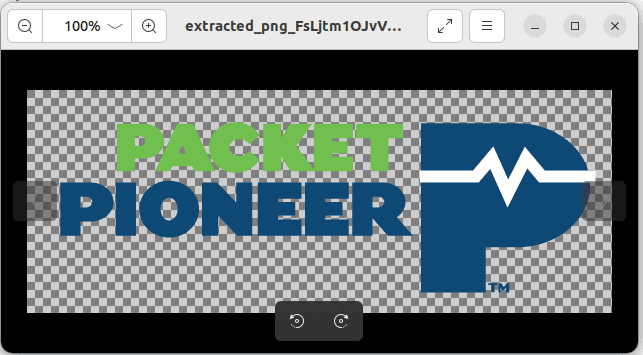
\includegraphics[width=0.5\linewidth]{images//extract_file/file_extract_3.png}
    \caption{PNG file}
    \label{fig:enter-label}
\end{figure}

\begin{itemize}
\item A TXT file has been successfully extracted from the network traffic.

 \end{itemize}
\begin{figure}[H]
    \centering
    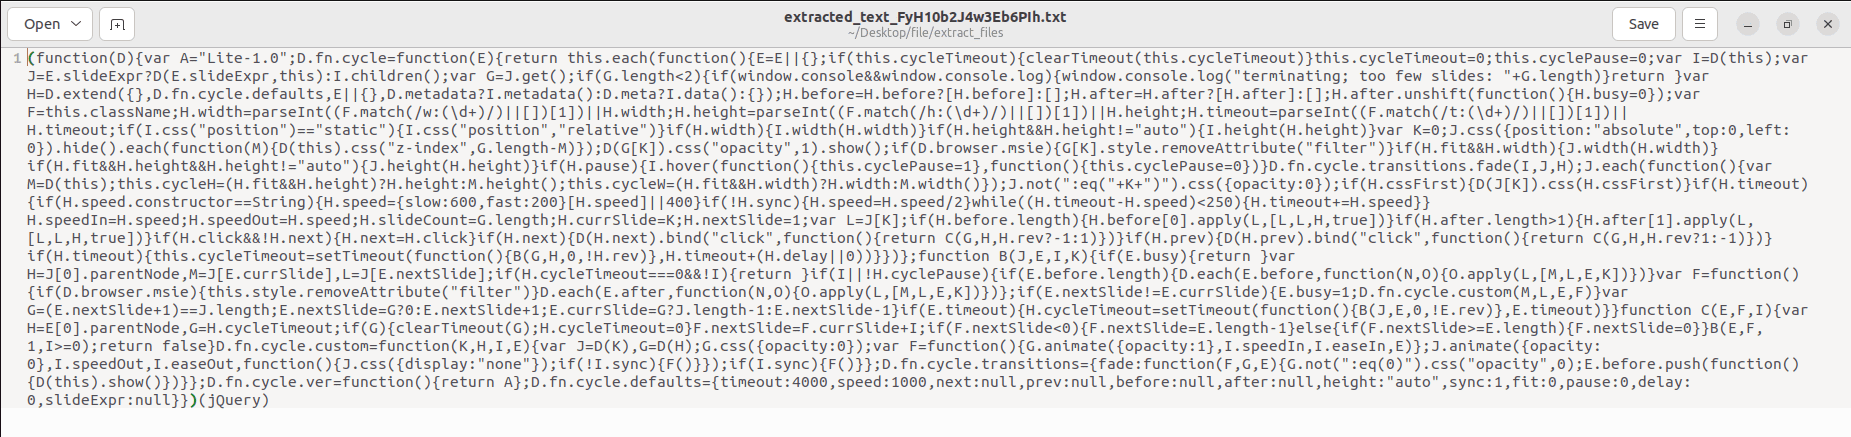
\includegraphics[width=1\linewidth]{images//extract_file/file_extract_4.png}
    \caption{TXT file}
    \label{fig:enter-label}
\end{figure}

\begin{itemize}
\item Additionally, the files.log file, which can be viewed in BRIM, provides an MD5 hash value for each extracted file, facilitating further analysis and verification of the files' integrity.

 \end{itemize}
\begin{figure}[H]
    \centering
    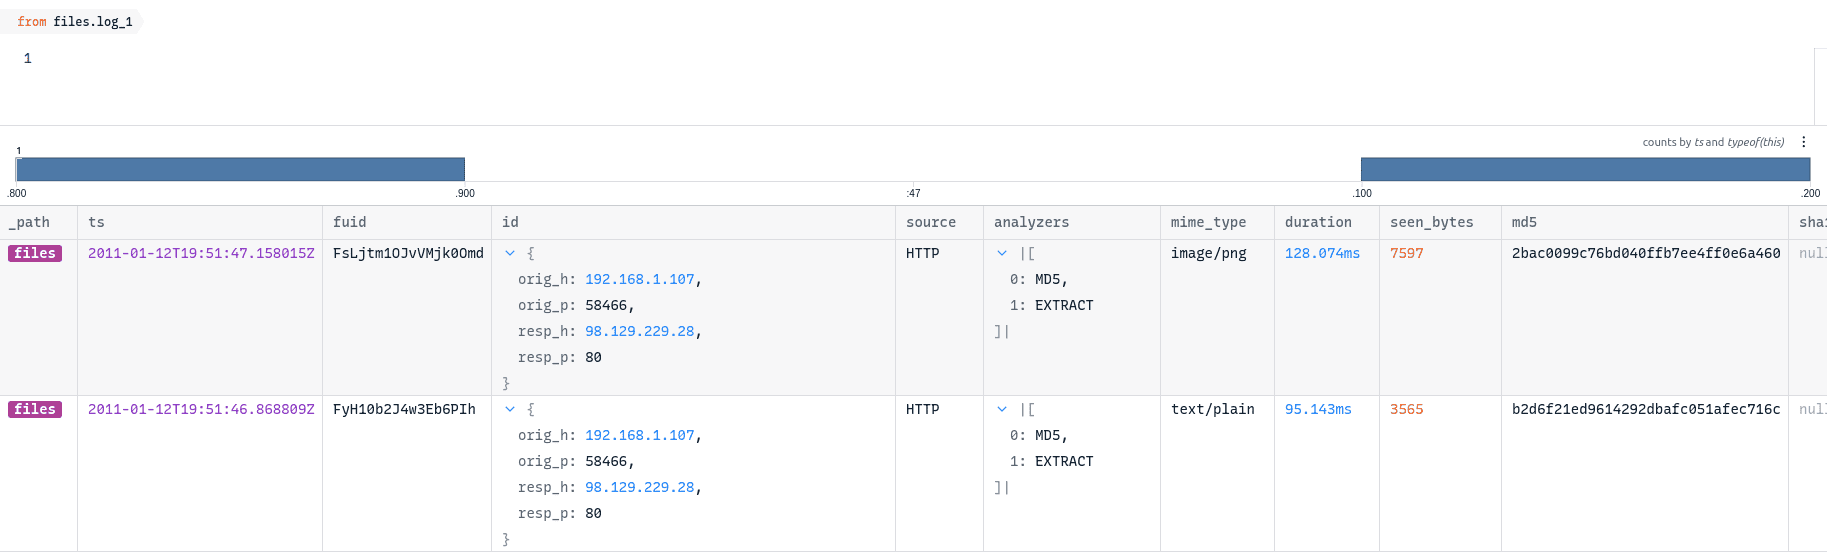
\includegraphics[width=1\linewidth]{images//extract_file/file_extract_5.png}
    \caption{files.log in BRIM}
    \label{fig:enter-label}
\end{figure}

